\section{Results: the \sig{} knockout}
\label{sec:results}

All numbers in this section are on the 9.56M-parameter models of Table~\ref{tab:arms}, judged by Lean alone, from the
evaluation with sample seed x0 unless stated. An analyst who had not written the experiment's code recounted every count
in this section from the raw files, with separate code, and re-checked the proofs in Lean. Numbers computed for this
paper are marked (\emph{this paper}); they are recomputed from those recounted files.

\subsection{No knockout seed acquired a family in 16 rounds}
\label{sec:primary}

\begin{table}[t]
\centering\small
\caption{Strict held-out theorems proved (of 106) per seed at r0 (end of pretraining), r8 and r16, and the families
acquired. x0 and x1 are two sample seeds; ``guided'' is the guided evaluation. Families: cc = converse contraposition,
nc = negated conditional, pe = Peirce, ps = Peirce sequent, em = excluded middle; families acquired already at r0 are
underlined. $\dagger$ = seeds from earlier runs (other GPU class and batch in rounds 1--8). The dose arm's other
evaluations are in Appendix~\ref{sec:checks}.}
\label{tab:primary}
\begin{tabular}{lrrrrrll}
\toprule
model & r0 & r8 & r16 x0 & r16 x1 & guided & acquired at r16 (x0) & gain r0$\to$r16 \\
\midrule
\Kfull{} s0$^\dagger$ & 18 & 38 & 42 & 43 & 44 & \underline{cc}, nc & 24 \\
\Kfull{} s1$^\dagger$ & 6 & 25 & 75 & 73 & 75 & cc, em, pe & 69 \\
\Kfull{} s2$^\dagger$ & 22 & 66 & 77 & 77 & 80 & \underline{cc}, nc, pe, ps & 55 \\
\Kfull{} s3 & 23 & 59 & 65 & 64 & 64 & \underline{cc}, nc, pe, ps & 42 \\
\Kfull{} s4 & 15 & 21 & 23 & 22 & 24 & \underline{cc} & 8 \\
\Kfull{} s5 & 18 & 19 & 33 & 34 & 33 & \underline{cc}, ps & 15 \\
\midrule
\Kko{} s0 & 0 & 0 & 0 & 0 & 0 & -- & 0 \\
\Kko{} s1 & 0 & 1 & 2 & 2 & 3 & -- (r20: 5; r24: 5) & 2 \\
\Kko{} s2 & 0 & 0 & 1 & 1 & 0 & -- & 1 \\
\Kko{} s3 & 0 & 0 & 0 & 0 & 0 & -- & 0 \\
\Kko{} s4 & 0 & 0 & 0 & 0 & 0 & -- & 0 \\
\Kko{} s5 & 0 & 0 & 2 & 1 & 2 & -- & 2 \\
\midrule
\Kdose{} s0 & 6 & 53 & 58 & & & cc, nc, pe, ps & 52 \\
\Kdose{} s1 & 18 & 33 & 39 & & & \underline{cc}, nc & 21 \\
\Kdose{} s2 & 8 & 28 & 30 & & & cc, nc & 22 \\
\bottomrule
\end{tabular}
\end{table}

No knockout seed acquired any classical family by r16; every full seed had at least one (Table~\ref{tab:primary},
Fig.~\ref{fig:endpoint}). This is the pre-registered primary indicator, 6/6 against 0/6, one-sided Boschloo
$p = 0.00024$. The same holds in the second sample seed, in the guided evaluation, and with the looser held-out sets
first pre-registered (178 theorems; they were replaced by the strict sets in a dated amendment after round 1 of the
first knockout ladder, because that base proved 136 of 155 generated ``classical'' targets using a $\neg\neg$ the
sequent supplied). The 0/6 bounds the per-seed rate at which this EI acquires a family from a \sig-free base below 0.39
(one-sided 95\%).

The indicator is a weak statement about RL, however. Converse contraposition is acquired \emph{before} RL on 5/6 full
bases (6/6 in the guided evaluation). Applied to the bases, the indicator already gives 5/6 against 0/6 ($p = 0.0032$),
or 6/6 against 0/6 in the guided evaluation ($p = 0.00024$). Per family, the pre-registered rule gives
\textsc{needs exposure} only for converse contraposition (6 vs 0 seeds; Holm-corrected over six families, 0.0015). It
gives \textsc{undetermined} for negated conditional, Peirce and the Peirce sequent (3 vs 0 each; $p = 0.034$, Holm 0.17)
and for excluded middle (1 vs 0), and \textsc{neither} for De Morgan, whose four strict members no model proves.

The comparisons specific to RL were not pre-registered. During RL, the full seeds gained 24, 69, 55, 42, 8 and 15 strict
held-out theorems and the knockout seeds 0, 2, 1, 0, 0 and 2: the arms do not overlap (exact one-sided Mann--Whitney
$U = 36$, $p = 0.0011$). Counting only families acquired between r0 and r16, it is 5/6 against 0/6 ($p = 0.0032$). The
old full seeds ran rounds 1--8 on other hardware. Restricted to the three new full seeds, it is 2/3 against 0/6
($p = 0.034$). On the training side, the knockout ladders proved none of the 123 strict training theorems in round 1
and only 0, 5, 1, 0, 0 and 2 of them by round 16. The full ladders went from 21, 1, 27, 17, 15 and 20 in round 1 to 49,
80, 86, 78, 33 and 36 (Fig.~\ref{fig:dynamics}a). No knockout ladder ever had proofs for half of any family's strict
training theorems.

\begin{figure}[t]
\centering
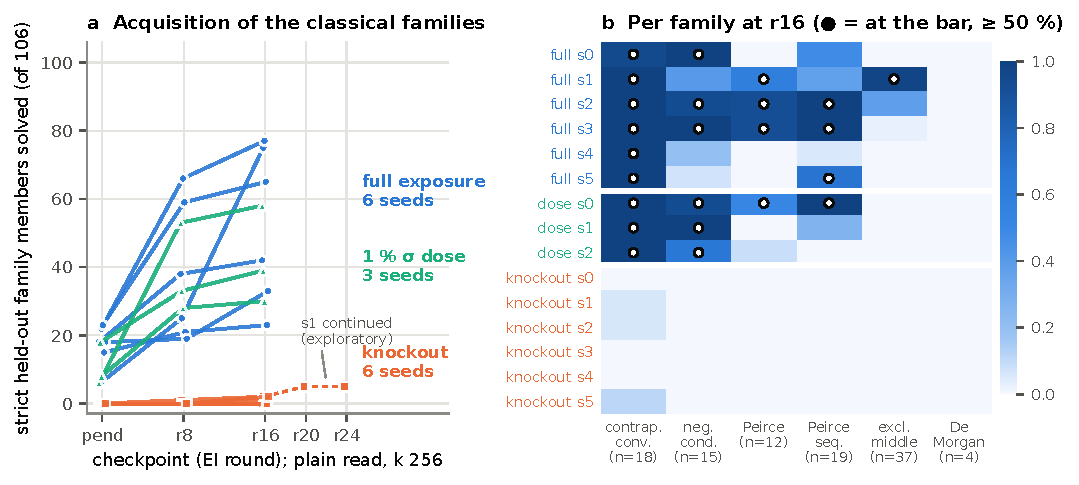
\includegraphics[width=\linewidth]{figures/fig1_endpoint.pdf}
\caption{\textbf{Per seed and per family.} (a) Strict held-out theorems proved at r0, r8 and r16; knockout seed 1 was
continued to r24 (dashed; exploratory). (b) Share of each family's strict held-out members proved at r16; a dot marks
an acquired family ($\geq 50\%$).}
\label{fig:endpoint}
\end{figure}

\subsection{One percent is enough}
\label{sec:dose}

The dose bases proved 6, 18 and 8 strict held-out theorems at r0, and 58, 39 and 30 at r16. All three acquired families
during RL; dose s1 had already acquired converse contraposition at r0. That is 3/3 against the knockout's 0/6
(Boschloo $p = 0.0033$; this arm was added by a dated amendment before it ran, and is exploratory). At r16 the dose seeds
lie inside the full arm's range (two-sided Mann--Whitney $p = 0.55$ with three seeds; \emph{this paper}). In round 1 the
dose bases wrote 223, 183 and 241 \sig{} proofs, and the free positive reductio from round 1 on. The new full seeds
wrote 635--885 \sig{} proofs and the knockout seeds 6--13. The dose changes the data around \sig{} far less than the
knockout removed. In \KTdose{}, \texttt{DN} appears in 4.24\% of records and $\neg$-introduction in 6.12\%, against 3.29\% and 5.19\% in \KTko{} and 13.73\% and 15.21\% in \KT{}. Classical-only theorems are 1.56\% of a 20,000-record sample, against 1.35\% and 4.17\% (\emph{this paper}, from the dose set's file). A second sample seed and a guided evaluation of the dose arm, run for this paper, agree. The second seed
proves 56, 39 and 30 strict theorems, and the guided evaluation proves 58 and 42 on seeds 0 and 1 (seed 2 pending). All three seeds acquire the same families
as in the first evaluation (Appendix~\ref{sec:checks}).

\subsection{\sig{} is rare in the knockout arm, not absent}
\label{sec:rare}

\paragraph{The bases, sampled about a million times.} We drew 1.1--1.5 million attempts from each knockout base, spread
over the 106 strict held-out theorems (about $10^4$ per theorem, with sampling on a theorem paused after its first
success in each block of 1,024). Five of the six bases proved strict theorems: seed 1 seven times, seed 4 three times,
seed 5 twice, and seeds 2 and 3 once each. Every success is a genuine \sig{} proof, and twelve of the fourteen are on
family members, eleven of them converse contraposition. Seed 3's single success is on the generated theorem
\texttt{la\_transfer\_916}. Pooled rates are 0 to $6\times10^{-6}$ per attempt; on the theorems with a success, the
per-theorem estimates are $7.5\times10^{-5}$ to $4.9\times10^{-4}$, each from one to three successes.

\paragraph{Certificates.} As pre-registered, pooled over the 106 theorems at each seed's $\Ktrain(16)$, only seed 0's
base is certified out of reach: 0 successes in 1.50 million attempts, $\mathrm{UB}_{95} = 1.99\times10^{-6} <
0.05/K = 2.14\times10^{-6}$ (Table~\ref{tab:certs}). Its certificate holds up to $K = 25{,}112$, 8\% above the budget,
and only at this one allocation and $N_{\mathrm{eval}}$. Pooled over the 105 family members alone, as the experiment
reported it, seed 3 is also certified; the difference is its success on \texttt{la\_transfer\_916}. No family is
certified for any seed: at this sampling the largest certifiable $K$ per family is 717--8,772. A pooled certificate
bounds the mean rate over the pool, not any theorem in it.

\begin{table}[t]
\centering\small
\caption{Knockout bases at large $k$, pooled over the 106 strict held-out theorems (the pre-registered pool), at each
seed's $K = \Ktrain(16)$. Certified out of reach if $\mathrm{UB}_{95} < 0.05/K$; $K_{\max} = 0.05/\mathrm{UB}_{95}$ is
the largest budget the data certify. In parentheses: the 105 family members only (excluding
\texttt{la\_transfer\_916}).}
\label{tab:certs}
\begin{tabular}{lrrrrc}
\toprule
knockout base & $K$ & attempts & successes & $K_{\max}$ & certified \\
\midrule
s0 & 23,322 & 1,504,600 & 0 (0) & 25,112 (24,892) & yes (yes) \\
s1 & 17,189 & 1,122,426 & 7 (6) & 4,268 (4,730) & no (no) \\
s2 & 20,907 & 1,350,143 & 1 (1) & 14,230 (14,106) & no (no) \\
s3 & 20,782 & 1,342,688 & 1 (0) & 14,152 (22,376) & no (yes) \\
s4 & 21,554 & 1,372,403 & 3 (3) & 8,850 (8,772) & no (no) \\
s5 & 22,297 & 1,432,256 & 2 (2) & 11,375 (11,275) & no (no) \\
\bottomrule
\end{tabular}
\end{table}

\paragraph{The ladders.} Every knockout ladder wrote \sig{} in round 1, 6--13 distinct proofs per ladder, on theorems
that supply $\neg\neg G$ or whose goal is a negation. Over their rounds, the fine-tuning mixes carried 844--4,428 such
self-written \sig{} records (2,948--9,140 \sigp{}). The free positive reductio was another matter. Over 16 rounds the
knockout ladders produced 0, 34, 4, 1, 2 and 16 distinct proofs using it, first in rounds never, 9, 12, 15, 15 and 2.
The full ladders produced 17,507--50,222 each, and the dose ladders 20,597--26,662, from round 1
(Fig.~\ref{fig:dynamics}b). EI thus trained on \sig{} in easy contexts from the start and did not carry the step to
the theorems that need it.

\begin{figure}[t]
\centering
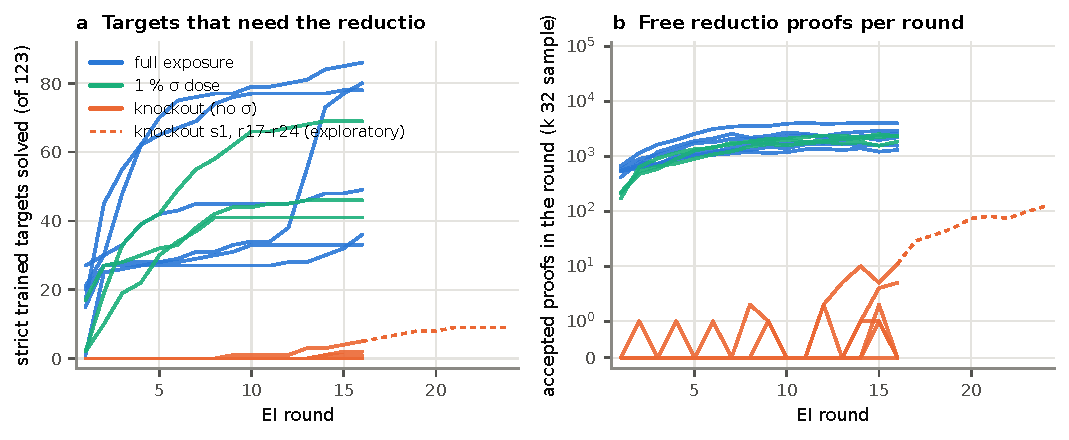
\includegraphics[width=\linewidth]{figures/fig2_dynamics.pdf}
\caption{\textbf{Ladder dynamics.} (a) Strict training theorems (of 123) with an accepted proof so far. (b) Accepted
proofs per round, in each round's $k=32$ sample over all 4,495 training theorems, that use a free positive reductio
(symmetric-log scale). Full and dose ladders write hundreds from round 1 and thousands later. Four knockout ladders
write a few, late. Knockout s1 (dashed beyond round 16) spreads it, from 11 in round 16 to 123 in round 24.}
\label{fig:dynamics}
\end{figure}

\paragraph{Beyond the waiting-time null (\emph{this paper}, post hoc).} Suppose each knockout ladder kept sampling the
123 strict training theorems at its base's pooled rate. It would then expect a first strict success after 47 (seed 1),
115 (seed 4), 180 (seed 5) and 340 (seed 2) rounds, and never for seeds 0 and 3. The expected number of seeds with a
strict success by round 16 is 0.55. Three had one: seed 1 in round 9, seeds 2 and 5 in round 14. Under the null that is
a $p = 0.006$ event. So EI did raise the knockout models' rate of the free positive reductio, presumably through the
\sig{} it practised on easier theorems, but not by enough to acquire a family. The two certified-on-105 bases (s0, s3)
never produced one.

\paragraph{Likelihood.} We scored the best known \sig{} proof of each of 101 strict held-out theorems under every
checkpoint, teacher-forced at $T=0.8$ (Fig.~\ref{fig:logp}). The proofs are the full ladders' own. At r0 the median
log-probability is $-15.4$ to $-20.9$ nats under the four full bases scored, $-18.9$ to $-25.3$ under the dose bases,
and $-26.0$ to $-36.0$ under the knockout bases. The arms overlap only between dose and knockout seed 1. The step that
costs most is the box that assumes $\neg G$: $-18.0$ to $-21.6$ nats under the knockout bases, $-10.5$ under full seed
0's base. From r0 to r16, two ladders move strongly toward these proofs (full s3 $+10.3$ nats, dose s0 $+16.6$). The
other full and dose ladders move $+1.7$ to $+4.3$, and the knockout ladders $-7.6$ to $+3.7$. Several knockout ladders
rise by 5--8.5 nats by r4 and fall back. Two caveats apply. The scores use one of the 33 line-numbering offsets, so
they understate a proof's probability by at most $\ln 33 \approx 3.5$ nats. And a knockout ladder that found its own
spelling (seed 1, below) need not raise these.

\begin{figure}[t]
\centering
\begin{minipage}{0.49\linewidth}
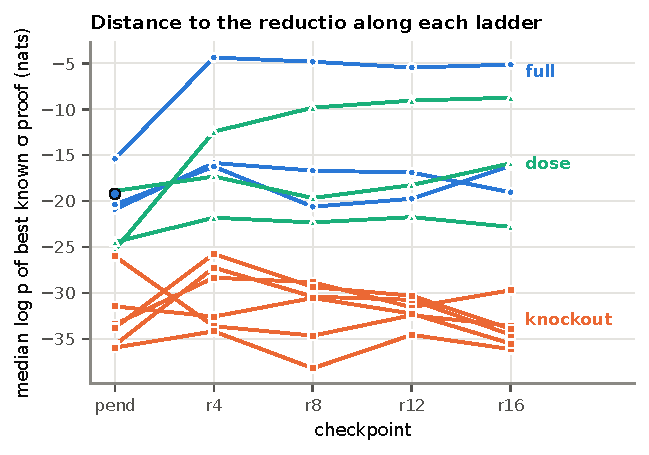
\includegraphics[width=\linewidth]{figures/fig3_logp.pdf}
\caption{Median log-probability of the best known \sig{} proof of the strict held-out theorems, along each ladder (one
line-numbering offset, $T=0.8$). The outlined point is full seed 0's base, whose ladder was not rescored.}
\label{fig:logp}
\end{minipage}\hfill
\begin{minipage}{0.49\linewidth}
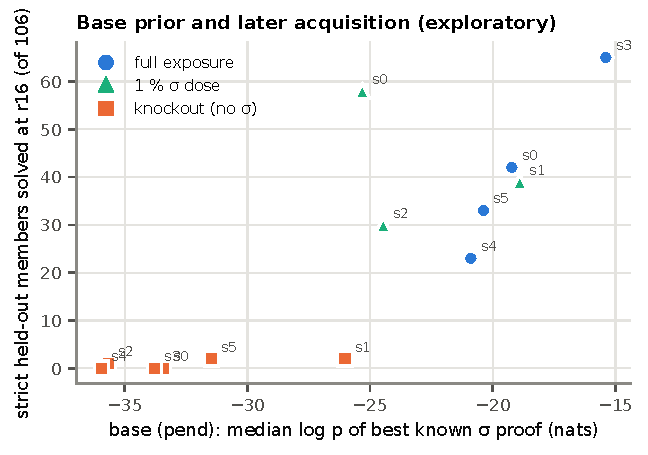
\includegraphics[width=\linewidth]{figures/fig6_prior.pdf}
\caption{Exploratory (\emph{this paper}): the base's median log-probability of known \sig{} proofs against strict
held-out theorems proved at r16, for the 13 ladders with a scored base.}
\label{fig:prior}
\end{minipage}
\end{figure}

\subsection{The one knockout ladder that moved}
\label{sec:ko-s1}

Knockout seed 1's free reductio kept spreading, so it was continued to round 24 (exploratory). Its free positive
reductio proofs per round rose from 11 in round 16 to 123 in round 24. From round 21 it had proofs for 9 of the 27
strict converse-contraposition training theorems, and it never went past 9 strict training theorems in all. It proved
the same five strict held-out theorems at r20 and r24, each more often: four converse-contraposition members and
\texttt{la\_transfer\_916}. The largest gain is on \texttt{la\_transfer\_1019}, from 0 to 32 to 214 successes in 256
attempts at r16, r20 and r24. No family was acquired. Its r20 proofs of these theorems take three routes: \sig{} (32
proofs), other \sigp{} (24) and the lemma route (7), a route absent from every pretraining set.

Was this elicitation of something the base already did? In the large-$k$ sample, the base proved four of its 18
converse-contraposition members, each one to three times in 7,168--10,240 attempts. That is within reach by the rate
definition, but every one is below $K$ attempts. Three of the four members the ladder proves (\texttt{1246},
\texttt{1460}, \texttt{2256}) are among them. The fourth, \texttt{1019}, had no base success in about $10^4$ attempts.
A re-sample of these members at $n \geq K$ without early stopping, run for this paper, is pending.

\subsection{What else the knockout changes}
\label{sec:side}

\paragraph{Data.} Removing \sigp{} records also thins its constituents. In \KTko{}, \texttt{DN} appears in 3.29\% of
records (13.73\% in \KT{}) and $\neg$-introduction in 5.19\% (15.21\%). Theorems with no intuitionistic proof fall from
4.17\% to 1.35\% of a 20,000-record sample; the rest use \texttt{DN} on a $\neg\neg$ that a premise or an assumption
supplies. Mean proof term size moves from 35.91 to 36.25 nodes. The knockout removes the composition's co-occurrence,
and also makes each constituent three to four times rarer.

\paragraph{General ability.} The knockout bases are 6.88 points worse at greedy decoding of 5,000 held-out generator
theorems (0.8829 vs 0.9517). The gap comes from the 679 theorems whose reference proof uses \sig{} (0.45 vs 0.96); on
the other 4,321 the knockout is 0.12 points better. With 256 attempts, though, the knockout bases also prove 4.3 fewer
of the 225 intuitionistic theorems of holdout250, and 4.0 fewer of textbook72's 53 (three full seeds against six
knockout seeds). By r16 the holdout250 gap closes (0.996 vs 0.996), while textbook72 keeps $-2.5$.

\paragraph{Gains elsewhere.} On the 322 evaluation theorems, RL's gain over what its own base reaches at RL's budget
(\dcov{} at $\Ktrain(16)$, with the base given 512 attempts and then at least $K$ on every theorem it failed) is $+37$,
$+36$ and $+32$ for full seeds s3--s5 and $+21$ to $+37$ for the knockout seeds: means 35.0 and 29.8, one-sided
Mann--Whitney $p = 0.13$ (\emph{this paper}). The knockout ladders are not clearly worse at RL in general, and they may
be somewhat worse. These sets are not netted against RL-free controls.

\paragraph{What this means for the interpretation.} Three things favour exposure to the composition over a general
deficit. The general costs are a few theorems out of hundreds, against a gap of 8--69 vs 0--2 strict theorems gained
during RL. The knockout ladders' gains elsewhere are comparable. And the dose arm restores acquisition while moving \texttt{DN} and
$\neg$-introduction by about one point each (\S\ref{sec:dose}). The design cannot separate exposure in pretraining from exposure
through replay during RL (\S\ref{sec:setup}).

\subsection{The base's prior predicts what RL acquires (exploratory)}
\label{sec:prior}

Across the 13 ladders with a scored base, the base's median log-probability of known \sig{} proofs is rank-correlated
with strict held-out theorems proved at r16 (Spearman $\rho = 0.88$; Fig.~\ref{fig:prior}). This is mostly the
difference between arms: $\rho = 0.39$ ($p = 0.38$) without the knockout. Within a ladder, the base's log-probability
of a member's best known proof predicts whether the member is proved at r16. The AUC is 0.92--0.95 on the four full
seeds with scored bases (pre-registered expectation $\geq 0.7$) and 0.85--0.86 on the three dose seeds. Comparing only
members of the same family, the AUC is 0.47--0.98 (full) and 0.28--0.60 (dose). The base's log-probability also
predicts \emph{when} a member is first proved in the ladder's per-round samples. The Spearman $\rho$ with the
first-solve round is $-0.69$ to $-0.87$ on the full seeds and $-0.61$ to $-0.72$ on the dose seeds, and $-0.33$ to
$-0.48$ within families on the full seeds (all \emph{this paper}). This agrees with reports that reference-solution
likelihood predicts later success \citep{schaeffer2025generative,shen2026chess} and that RL gains concentrate where the
base already succeeds sometimes \citep{zhang2025interplay}.

\subsection{Two nulls}
\label{sec:nulls}

\paragraph{One seeded round.} From each knockout r16 checkpoint we ran one more EI round, with and without four copies
of one free positive reductio proof written by knockout seed 1's base. Seeded minus control was $+0$, $+0$, $+2$, $+0$
and $+0$ strict family members on seeds 0, 1, 2, 3 and 5 (seed 4 not run); seed 2's two were single successes in 256
attempts (one-sided exact $p = 0.25$). One round is too short to test seeding. In an earlier, smaller organism, a single
injected proof ignited a similar pattern within one to two rounds (\S\ref{sec:discussion}).

\paragraph{Power sampling.} Metropolis--Hastings sampling from $p^\alpha$ of the full and knockout bases
\citep{karan2025power} ($\alpha = 2$, 4; 32 chains per theorem) proved none of the theorems RL r8 proves beyond the base's
reach (0/33, 0/27), and none of the 106 strict theorems for knockout bases s0 and s1. Plain sampling with the same decoded
tokens proved 1--2. The sampler also failed its positive control: on 17 theorems the base proves rarely, it proved 0/17,
where plain sampling at the same tokens proved 6/17 ($T=0.8$) and 13/17 ($T=1.0$). This is a null for this sampler at
these settings, not for sharpening. It agrees with the finding that practical power samplers do not reach $p^\alpha$ at
realistic budgets \citep{talwar2026power}. Details are in Appendix~\ref{app:power}.

\subsection{Robustness}
\label{sec:robust}

The independent re-check accepted every stored knockout proof of a strict theorem in Lean 4.34.1 (448/448), the version
used in the loop. It rejected all 150 re-submitted Lean rejections, all 60 proofs paired with the wrong theorem, all 40
strict knockout proofs with \texttt{Classical.byContradiction} removed, and \texttt{sorry}. Every rejection in the
experiment was the pre-filter's, so the pre-filter's false-reject rate matters. Re-checking 150 rejections per reason
for its 13 reasons gave 0 accepted, a 95\% bound of 2.0\% per reason. This paper Lean-checked every one of the 222,135
pre-filter rejections in knockout seed 1's ladder (rounds 1--16; 22,522 of them on a by-contradiction step); the result is pending.
Cut-offs (a step over 512 tokens or a proof over 96 steps) can only hide successes. On the strict theorems at r16 they
affect 0.04--4.97\% of knockout attempts, 0.11--2.89\% of full and 0.68--8.84\% of dose attempts. A paired re-evaluation
with doubled caps, run for this paper, moves the counts by at most one theorem so far and changes no verdict
(Appendix~\ref{sec:checks}). The training theorems share no renaming class with any evaluation
set, and no pretraining set shares one with the 106 strict theorems.
